\documentclass{article}
\usepackage{amsmath}
\usepackage[utf8]{inputenc}
\usepackage[margin=2cm]{geometry} 
\usepackage{graphicx}
\usepackage{placeins}
\usepackage[skip=10pt plus1pt, indent=40pt]{parskip}
\usepackage{float}
\usepackage{booktabs}
\usepackage{multicol}
\usepackage{gensymb}
\usepackage{amsmath}
\usepackage{hyperref}
\hypersetup{
    colorlinks=true,
    linkcolor=blue,
    filecolor=blue,
    citecolor=black,
    urlcolor=cyan
    }


\begin{document}

\title{Indice di rifrazione del plexiglass e focale di una lente divergente}
\author{Alessia Di Nino, Alessandra Natì (corso B, gruppo B 1-2)}
\date{16 Marzo 2023}
\maketitle

\section{Indice di rifrazione del plexiglass}

\vspace{1em}

\subsection{Introduzione}
\subsubsection{Cenni teorici} %alessia
Se un raggio di luce passa da un mezzo con indice di rifrazione $n_1$ ad uno con
indice di rifrazione $n_2$, gli angoli di incidenza $\theta_i$ e di rifrazione $\theta_r$ sono legati tra di
loro dalla legge di Snell: 

\begin{equation}
    n_1sin(\theta_i)=n_2sin(\theta_r)
\end{equation}

In questo esperimento, in particolare, si considera $n_1 \sim 1$, indice di rifrazione dell'aria e $n_2$ indice di rifrazione del plexiglass. Inoltre, $\theta_i$ è l'angolo formato tra il raggio incidente e la normale alla superficie di separazione tra i due mezzi.
%spiegare perché si considera indice di rifrazione dell'aria pari a 1 (approssimazione): n_aria - 1 << sigma_n\n
\begin{figure} [H]
    \centering
    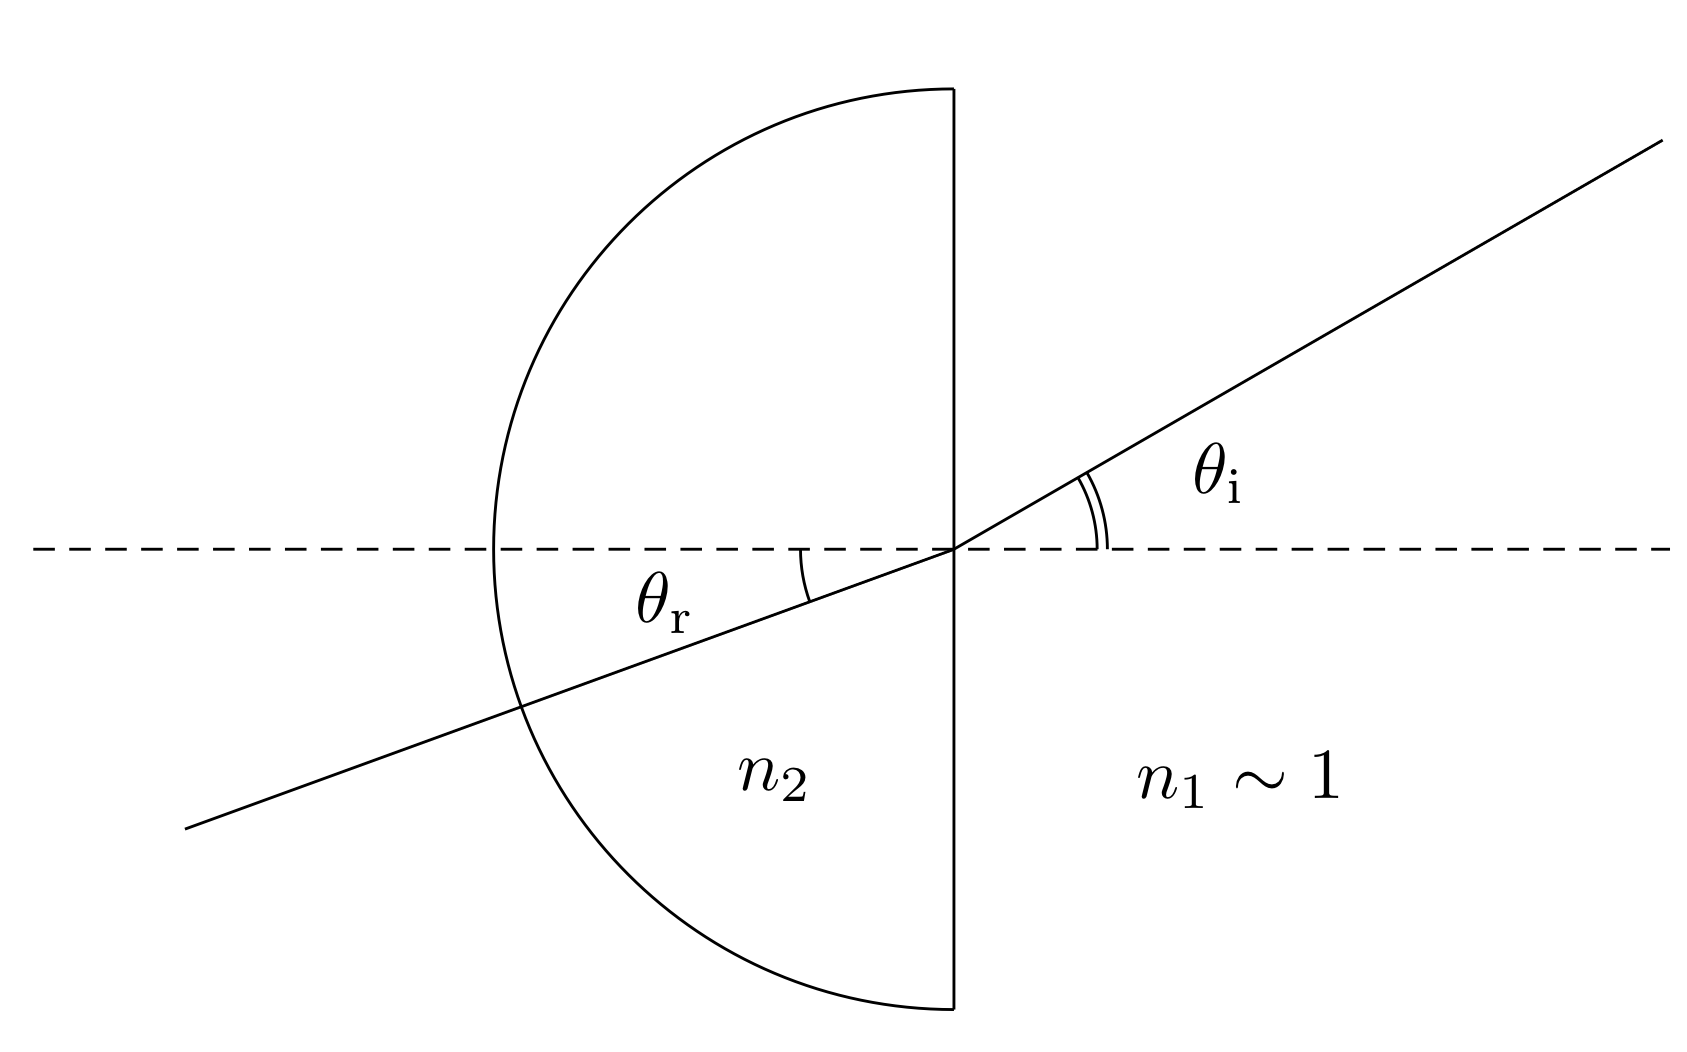
\includegraphics[width=10cm]{schema_lenti(1).png}
    \caption{Schematizzazione delle grandezze in gioco nell'esperimento}
    \label{fig:my_label}
\end{figure}

Oltre la legge di Snell, la seguente espressione permette di misurare l'indice di rifrazione di un mezzo grazie all'angolo limite: si dice angolo limite l'angolo oltre il quale avviene riflessione totale, visibile dall'avvicinarsi, fino a scomparsa, del raggio rifratto all'asse ottico: 

\begin{equation}
    n = \frac{1}{sin \theta_i}
    \label{n}
\end{equation}
\FloatBarrier

dove $\theta_i$ è l'angolo di incidenza (che è uguale a quello di riflessione).

\vspace{1em}

\subsubsection{Scopo dell'esperienza} %alessandra
Obiettivo centrale di questa esperienza è proprio quello di misurare l'indice di rifrazione del plexiglass.

\vspace{2em}

\subsection{Metodi}
\subsubsection{Apparato sperimentale} %alessia
\begin{enumerate}
    \item Strumenti utilizzati:
    \begin{itemize}
        \item griglia quadrettata di risoluzione 1 quadretto ($2mm$);
        \item pennarelli (per segnare le coppie di angolo di incidenza e rifrazione).
    \end{itemize}

    \item Materiale a disposizione:
    \begin{itemize}
        \item banco ottico con sorgente luminosa;
        \item fenditura;
        \item lente convergente (di potere diottrico +12);
        \item semicilindro di plexiglass;
        \item supporto per il semicilindro di plexiglass.
    \end{itemize}
\end{enumerate}
\FloatBarrier

\begin{figure} [H]
\begin{minipage}[b]{8.5cm}
\centering
\includegraphics[width=6cm]{2.jpg}
\caption{Banco ottico e lente convergente}
\end{minipage}
\ \hspace{2mm} \hspace{3mm} \
\begin{minipage}[b]{8.5cm}
\centering
\includegraphics[width=6cm]{1.jpg}
\caption{Sorgente luminosa e fenditura}
\end{minipage}
\end{figure}
\FloatBarrier

\begin{figure} [H]
    \centering
    \includegraphics[width=12cm]{4.jpg}
    \caption{Semicilindro di plexiglass e griglia}
    \label{fig:my_label}
\end{figure}

\begin{figure} [H]
    \centering
    \includegraphics[width=12cm]{3.jpg}
    \caption{Apparato strumentale intero}
    \label{fig:my_label}
\end{figure}

\vspace{1em}

\subsubsection{Descrizione delle misure} %alessandra
Per condurre le misure, abbiamo posto il piattino (base del cilindro di plexiglass) ad una distanza dalla sorgente di luce tale che il raggio incidente (e rifratto) fosse sottile al punto da poter segnare correttamente il punto di incidenza e di rifrazione sulla griglia. La griglia infatti è stato uno strumento fondamentale per la buona riuscita dell'esperimento: sul cerchio disegnato su di essa abbiamo segnato a coppie -con colori diversi così da distinguerle- il punto in cui la luce colpiva il semicilindro in plexiglass e quello corrispondente in cui invece la luce veniva rifratta. Il procedimento è stato ripetuto circa 10 volte facendo ruotare il foglio curandoci sempre del fatto che la luce colpisse il centro del semicilindro. Di seguito, abbiamo misurato la distanza (in quadretti) di ogni punto dalla normale alla superficie di incidenza (distanza che, per trigonometria, è espressa dalla legge $r sin \theta$, dove r è il raggio del cerchio della griglia e $\theta$ è alternativamente l'angolo di incidenza o di rifrazione), ottenendo i seguenti dati:

\begin{center}
    \begin{tabular}{c|c}
    \toprule
        $r sin \theta_i \pm 1$ [quadretti] & $r sin \theta_r \pm 1$ [quadretti]  \\
     \midrule
        1 & 1\\
    \midrule
    5 & 3\\
    \midrule
    10 & 7\\
    \midrule
    16 & 11\\
    \midrule
    19 & 14\\
    \midrule
    23 & 16\\
    \midrule
    27 & 19\\
    \midrule
    30 & 22\\
    \midrule
    33 & 23\\
    \midrule
    34 & 25\\
    \bottomrule
    \end{tabular}
\end{center}
%l'errore va diviso per rad 12 per ottenere quello statistico
Inoltre, abbiamo misurato l'indice di rifrazione anche sfruttando l'angolo limite: abbiamo fatto incidere il raggio, questa volta, sulla superficie curva del semicilindro e abbiamo fatto girare il supporto fino al raggiungimento dell'angolo limite.

\begin{figure} [H]
    \centering
    \includegraphics[width=8cm]{IMG_7193.jpeg}
    \caption{Angolo limite}
    \label{fig:my_label}
\end{figure}

Abbiamo misurato la distanza dalla normale alla superficie del punto d'intersezione tra raggio incidente e cerchio della griglia (29 $\pm 1$ [quadretti)]); abbiamo poi misurato anche il raggio del cerchio interno alla griglia (41 $\pm 1$ [quadretti)]). Dalla formula \eqref{n}, si ottiene:

\begin{center}   
$n_{plexiglass} = 1.41 \pm 0.04$
\end{center}

\vspace{1em}

\subsubsection{Analisi dei dati} %alessia
I dati raccolti sono stati analizzati tramite la funzione curve\_fit() di Python realizzando, per l'appunto, il grafico di best fit  e il grafico dei residui.\\
Abbiamo fatto un fit lineare dei dati da cui ci aspettavamo che il coefficiente angolare fosse proprio l'indice di rifrazione cercato e che l'intercetta fosse 0 (poichè, appunto, la legge di Snell descrive un modello in cui $rsin\theta_i = rsin\theta_r$ a meno di un fattore). Dall'analisi risultano i seguenti parametri di best-fit:

\begin{center}
    \begin{tabular}{c|c}
    \toprule
    $\hat{n_2}$ & $1.38 \pm 0.03$  \\
    \midrule
    $\hat{q}$ & $0.4 \pm 0.5$ \\
    \midrule
    $\chi^2$ & 4.0\\
    \midrule
    dof & 7\\
    \bottomrule
\end{tabular}
\end{center}

\begin{figure} [H]
    \centering
    \includegraphics[width=15cm]{fit-res.pdf}
    \caption{Grafico di best fit e grafico dei residui}
    \label{fig:my_label}
\end{figure}

\vspace{2em}

\subsection{Conclusioni} %alessandra
In conclusione, è possibile affermare che il fit sia buono per una serie di commenti:

\begin{itemize}
    \item l'intercetta del grafico di best - fit è compatibile con zero;
    \item nel grafico dei residui, i dati oscillano attorno allo zero per meno di una barra d'errore; %anche se questo, in generale, non è necessariamente il segno di un buon fit
    \item nonostante il valore di best fit per l'indice di rifrazione del plexiglass da noi ottenuto ($1.38 \pm 0.03$) non sia compatibile con il valore tabulato di 1.52, lo è tuttavia con il valore dell'indice di rifrazione misurato mediante il metodo dell'angolo limite (($1.41 \pm 0.04$): questo potrebbe indicare, per esempio, aver utilizzato per l'esperimento un materiale diverso rispetto a quello con cui si è misurato il valore tabulato;
    \item il $\chi^2$ deve valere in media $\nu$, cioè il numero di gradi di libertà (dato dalla differenza tra il numero di dati -nel nostro caso 10- e il numero di paramentri liberi, ovvero 2 -l'indice di rifrazione e l'intercetta), con una deviazione standard di $\sigma = \sqrt{2\nu}$, che è uguale a 4. Il $\chi^2$ da noi misurato rientra in tale intervallo ed è dunque indice della buona riuscita del fit.
\end{itemize}

\end{document}